\subsubsection{Device-interaction}

\begin{center}
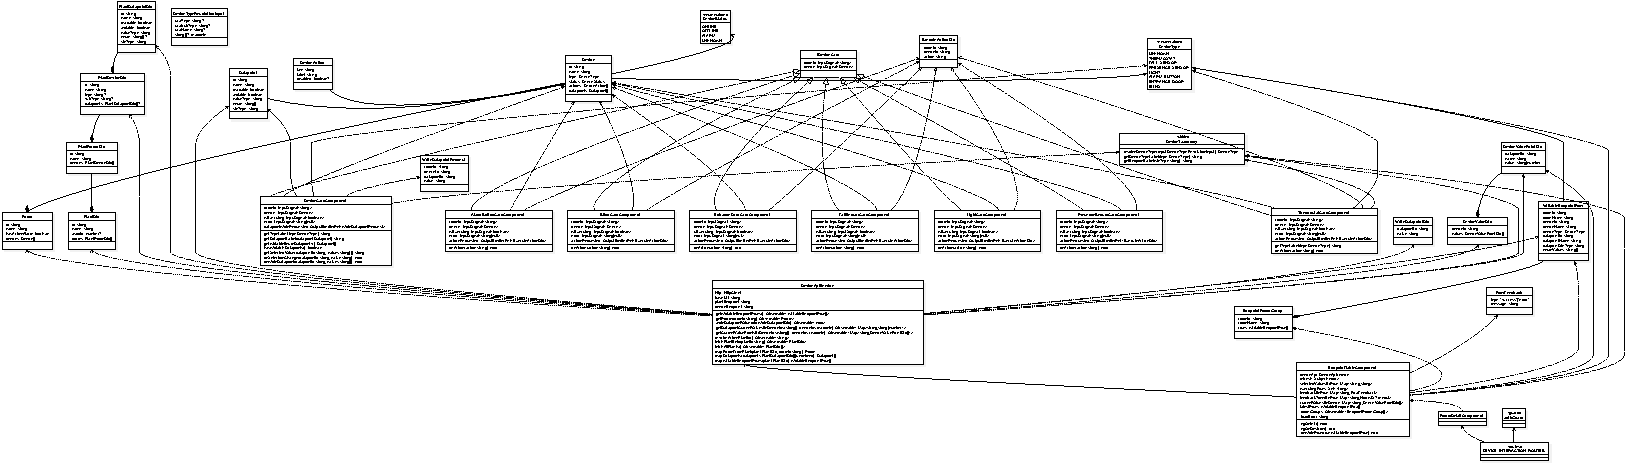
\includegraphics[width=\textwidth]{./frontend/device-interaction/device-interaction.pdf}
\captionof{figure}{Diagramma delle classi del modulo Device interaction}
\end{center}


\addAtr{+}{roomId: InputSignal$<$string$>$}{Segnale di input obbligatorio contenente l'identificativo della stanza a cui appartiene il dispositivo.}
\addAtr{+}{device: InputSignal$<$Device$>$}{Segnale di input obbligatorio contenente i dati del dispositivo da visualizzare.}
\addAtr{+}{isExecuting: InputSignal$<$boolean$>$}{Segnale di input che indica se è in corso l'esecuzione di un'azione sul dispositivo.}
\addAtr{+}{error: InputSignal$<$string $|$ null$>$}{Segnale di input contenente l'eventuale messaggio di errore da visualizzare.}
\addAtr{+}{actionRequested: OutputEmitterRef$<$ExecuteActionDto$>$}{Evento emesso quando l'utente richiede l'esecuzione di un'azione sul dispositivo.}
\addMet{+}{onAction(action: string) : void}{Emette l'evento \texttt{actionRequested} con i dati necessari all'esecuzione dell'azione richiesta.}
\makeCl{AlarmButtonCardComponent}{Componente Angular che rappresenta una card per un dispositivo di tipo pulsante allarme. Implementa IDeviceCard ed emette le azioni richieste dall'utente verso il componente padre.}

\addAtr{+}{roomId: InputSignal$<$string$>$}{Segnale di input obbligatorio contenente l'identificativo della stanza a cui appartiene il dispositivo.}
\addAtr{+}{device: InputSignal$<$Device$>$}{Segnale di input obbligatorio contenente i dati del dispositivo da visualizzare.}
\addAtr{+}{isExecuting: InputSignal$<$boolean$>$}{Segnale di input che indica se è in corso l'esecuzione di un'azione sul dispositivo.}
\addAtr{+}{error: InputSignal$<$string $|$ null$>$}{Segnale di input contenente l'eventuale messaggio di errore da visualizzare.}
\addAtr{+}{actionRequested: OutputEmitterRef$<$ExecuteActionDto$>$}{Evento emesso quando l'utente richiede l'esecuzione di un'azione sul dispositivo.}
\addMet{+}{onAction(action: string) : void}{Emette l'evento \texttt{actionRequested} con i dati necessari all'esecuzione dell'azione richiesta.}
\makeCl{BlindCardComponent}{Componente Angular che rappresenta una card per un dispositivo di tipo tapparella. Implementa IDeviceCard ed emette le azioni richieste dall'utente verso il componente padre.}

\addAtr{+}{roomId: InputSignal$<$string$>$}{Segnale di input obbligatorio contenente l'identificativo della stanza a cui appartiene il dispositivo.}
\addAtr{+}{device: InputSignal$<$Device$>$}{Segnale di input obbligatorio contenente i dati del dispositivo da visualizzare.}
\addAtr{+}{isExecuting: InputSignal$<$boolean$>$}{Segnale di input che indica se è in corso l'esecuzione di un'operazione sul dispositivo.}
\addAtr{+}{error: InputSignal$<$string $|$ null$>$}{Segnale di input contenente l'eventuale messaggio di errore da visualizzare.}
\addAtr{+}{datapointWriteRequested: OutputEmitterRef$<$WriteDatapointRequest$>$}{Evento emesso quando l'utente richiede la scrittura di un valore su un datapoint del dispositivo.}
\addAtr{-}{selectedValues: Map$<$string, string$>$}{Mappa che associa l'identificativo di ciascun datapoint al valore attualmente selezionato dall'utente.}
\addMet{+}{getTypeLabel(type: DeviceType) : string}{Restituisce l'etichetta localizzata corrispondente al tipo di dispositivo specificato.}
\addMet{+}{getDatapointLabel(datapoint: Datapoint) : string}{Restituisce l'etichetta localizzata corrispondente al tipo SFE del datapoint specificato.}
\addMet{+}{getWritableEnumDatapoints() : Datapoint[]}{Restituisce i datapoint del dispositivo che sono scrivibili e hanno valori enumerati disponibili.}
\addMet{+}{hasWritableDatapoints() : boolean}{Verifica se il dispositivo possiede almeno un datapoint scrivibile con valori enumerati.}
\addMet{+}{getSelectedValue(datapointId: string, values: string[]) : string}{Restituisce il valore selezionato per il datapoint specificato, inizializzandolo al primo valore disponibile se non ancora impostato.}
\addMet{+}{onSelectionChange(datapointId: string, value: string) : void}{Aggiorna il valore selezionato per il datapoint specificato nella mappa interna.}
\addMet{+}{onWriteDatapoint(datapointId: string, values: string[]) : void}{Emette l'evento datapointWriteRequested con il valore selezionato per il datapoint, se non è già in corso un'esecuzione.}
\makeCl{DeviceCardComponent}{Componente Angular che rappresenta una card generica per un dispositivo, con supporto alla lettura e scrittura dei datapoint enumerati. Implementa IDeviceCard e gestisce internamente la selezione dei valori da inviare al componente padre tramite eventi.}

\addAtr{-}{CURRENT\_VALUES\_POLL\_MS: number}{Costante statica che definisce l'intervallo in millisecondi tra un polling dei valori correnti e il successivo.}
\addAtr{-}{deviceApi: DeviceApiService}{Servizio utilizzato per effettuare le chiamate API relative ai dispositivi e ai loro datapoint.}
\addAtr{-}{refresh\$: Subject$<$void$>$}{Subject utilizzato per innescare il ricaricamento della lista delle righe endpoint.}
\addAtr{-}{selectedValuesByRow: Map$<$string, string$>$}{Mappa che associa la chiave di ciascuna riga al valore attualmente selezionato dall'utente.}
\addAtr{-}{executingRows: Set$<$string$>$}{Insieme delle chiavi delle righe per cui è in corso l'invio di un comando.}
\addAtr{-}{feedbackByRow: Map$<$string, RowFeedback$>$}{Mappa che associa la chiave di ciascuna riga al relativo feedback di esito operazione.}
\addAtr{-}{feedbackTimerByRow: Map$<$string, ReturnType$>$}{Mappa che associa la chiave di ciascuna riga al timer di auto-cancellazione del feedback.}
\addAtr{-}{currentValuesByDevice: Map$<$string, DeviceValuePointDto[]$>$}{Mappa che associa l'identificativo di ciascun dispositivo ai suoi valori correnti letti dal backend.}
\addAtr{-}{latestRows: WritableEndpointRow[]}{Ultima lista di righe endpoint caricata, utilizzata per il polling dei valori correnti.}
\addAtr{-}{activePlantChangeSubscription: Subscription $|$ null}{Sottoscrizione all'evento di cambio impianto attivo, gestita per il corretto cleanup.}
\addAtr{-}{currentValuesPollingSubscription: Subscription $|$ null}{Sottoscrizione al polling periodico dei valori correnti, gestita per il corretto cleanup.}
\addAtr{+}{roomGroups\$: Observable$<$EndpointRoomGroup[]$>$}{Stream reattivo che emette la lista delle righe endpoint raggruppate per stanza, aggiornandosi ad ogni refresh.}
\addAtr{+}{loadError: string}{Messaggio di errore da visualizzare in caso di fallimento nel caricamento delle righe endpoint.}
\addMet{+}{ngOnInit() : void}{Inizializza la sottoscrizione agli eventi di cambio impianto e avvia il polling periodico dei valori correnti.}
\addMet{+}{ngOnDestroy() : void}{Cancella le sottoscrizioni attive e i timer di feedback per prevenire memory leak.}
\addMet{+}{trackByGroup(\_ : number, group: EndpointRoomGroup) : string}{Restituisce l'identificativo della stanza per il tracking delle righe del gruppo nel template.}
\addMet{+}{trackByRow(\_ : number, row: WritableEndpointRow) : string}{Restituisce la chiave univoca della riga per il tracking nel template.}
\addMet{+}{getTypeLabel(type: DeviceType) : string}{Restituisce l'etichetta localizzata corrispondente al tipo di dispositivo specificato.}
\addMet{+}{getEndpointLabel(row: WritableEndpointRow) : string}{Restituisce l'etichetta localizzata corrispondente al tipo SFE del datapoint della riga.}
\addMet{+}{getCurrentValue(row: WritableEndpointRow) : string}{Restituisce il valore corrente del datapoint della riga, cercando prima per id esatto, poi per corrispondenza semantica e infine per primo valore disponibile.}
\addMet{+}{getSelectedValue(row: WritableEndpointRow) : string}{Restituisce il valore selezionato per la riga specificata, usando il primo valore enumerato come fallback.}
\addMet{+}{onSelectionChange(row: WritableEndpointRow, value: string) : void}{Aggiorna il valore selezionato per la riga specificata nella mappa interna.}
\addMet{+}{isRowExecuting(row: WritableEndpointRow) : boolean}{Verifica se è in corso l'invio di un comando per la riga specificata.}
\addMet{+}{getRowFeedback(row: WritableEndpointRow) : RowFeedback $|$ null}{Restituisce il feedback di esito operazione per la riga specificata, o \texttt{null} se non presente.}
\addMet{+}{onWriteRow(row: WritableEndpointRow) : void}{Invia il valore selezionato per la riga al backend, aggiornando il feedback e innescando il refresh in caso di successo.}
\addMet{-}{groupRowsByRoom(rows: WritableEndpointRow[]) : EndpointRoomGroup[]}{Raggruppa le righe endpoint per stanza, restituendo una lista di gruppi ordinati per ordine di inserimento.}
\addMet{-}{buildRowKey(row: WritableEndpointRow) : string}{Costruisce una chiave univoca per una riga combinando gli identificativi di stanza, dispositivo e datapoint.}
\addMet{-}{clearRowFeedback(rowKey: string) : void}{Rimuove il feedback e annulla il timer di auto-cancellazione per la riga specificata.}
\addMet{-}{setRowFeedback(rowKey: string, type: RowFeedback['type'], message: string) : \\ void}{Imposta il feedback per la riga specificata e pianifica la sua rimozione automatica dopo 5 secondi.}
\addMet{-}{subscribeToActivePlantChanges() : void}{Sottoscrive l'evento di cambio impianto attivo per resettare lo stato e ricaricare le righe.}
\addMet{-}{startCurrentValuesPolling() : void}{Avvia il polling periodico dei valori correnti dei dispositivi all'intervallo definito dalla costante statica.}
\addMet{-}{loadCurrentValues(rows: ReadonlyArray$<$WritableEndpointRow$>$) : Observable$<$void$>$}{Recupera i valori correnti per tutti i dispositivi presenti nelle righe fornite e aggiorna la mappa interna.}
\addMet{-}{getSemanticCandidates(row: WritableEndpointRow) : Set$<$string$>$}{Restituisce un insieme di chiavi normalizzate da usare per la ricerca semantica del valore corrente di un datapoint.}
\addMet{-}{convertCmdToState(value: string) : string}{Converte una chiave di tipo comando nella corrispondente chiave di tipo stato sostituendo il suffisso \texttt{cmd} con \texttt{state}.}
\addMet{-}{normalizeKey(value: string $|$ undefined) : string}{Normalizza una stringa rimuovendo caratteri speciali e convertendo in minuscolo per confronti semantici.}
\addMet{-}{syncSelectedValues(rows: ReadonlyArray$<$WritableEndpointRow$>$) : void}{Sincronizza la mappa dei valori selezionati con le righe correnti, aggiungendo nuove righe e rimuovendo quelle non più presenti.}
\addMet{-}{resetTransientState() : void}{Azzera tutto lo stato transitorio del componente, inclusi valori selezionati, esecuzioni in corso, feedback e valori correnti.}
\addMet{-}{clearAllRowFeedback() : void}{Cancella tutti i timer di feedback attivi e svuota le mappe di feedback.}
\makeCl{EndpointTableComponent}{Componente Angular che visualizza una tabella di endpoint scrivibili raggruppati per stanza, con supporto alla lettura dei valori correnti tramite polling e all'invio di comandi con feedback visivo. Gestisce il refresh automatico al cambio di impianto attivo e il cleanup delle sottoscrizioni al momento della distruzione.}

\addAtr{+}{roomId: InputSignal$<$string$>$}{Segnale di input obbligatorio contenente l'identificativo della stanza a cui appartiene il dispositivo.}
\addAtr{+}{device: InputSignal$<$Device$>$}{Segnale di input obbligatorio contenente i dati del dispositivo da visualizzare.}
\addAtr{+}{isExecuting: InputSignal$<$boolean$>$}{Segnale di input che indica se è in corso l'esecuzione di un'azione sul dispositivo.}
\addAtr{+}{error: InputSignal$<$string $|$ null$>$}{Segnale di input contenente l'eventuale messaggio di errore da visualizzare.}
\addAtr{+}{actionRequested: OutputEmitterRef$<$ExecuteActionDto$>$}{Evento emesso quando l'utente richiede l'esecuzione di un'azione sul dispositivo.}
\addMet{+}{onAction(action: string) : void}{Emette l'evento actionRequested con i dati necessari all'esecuzione dell'azione richiesta.}
\makeCl{EntranceDoorCardComponent}{Componente Angular che rappresenta una card per un dispositivo di tipo porta d'ingresso. Implementa IDeviceCard ed emette le azioni richieste dall'utente verso il componente padre.}

\addAtr{+}{roomId: InputSignal$<$string$>$}{Segnale di input obbligatorio contenente l'identificativo della stanza a cui appartiene il dispositivo.}
\addAtr{+}{device: InputSignal$<$Device$>$}{Segnale di input obbligatorio contenente i dati del dispositivo da visualizzare.}
\addAtr{+}{isExecuting: InputSignal$<$boolean$>$}{Segnale di input che indica se è in corso l'esecuzione di un'azione sul dispositivo.}
\addAtr{+}{error: InputSignal$<$string $|$ null$>$}{Segnale di input contenente l'eventuale messaggio di errore da visualizzare.}
\addAtr{+}{actionRequested: OutputEmitterRef$<$ExecuteActionDto$>$}{Evento emesso quando l'utente richiede l'esecuzione di un'azione sul dispositivo.}
\addMet{+}{onAction(action: string) : void}{Emette l'evento actionRequested con i dati necessari all'esecuzione dell'azione richiesta.}
\makeCl{FallSensorCardComponent}{Componente Angular che rappresenta una card per un dispositivo di tipo sensore di caduta. Implementa IDeviceCard ed emette le azioni richieste dall'utente verso il componente padre.}

\addAtr{+}{roomId: InputSignal$<$string$>$}{Segnale di input obbligatorio contenente l'identificativo della stanza a cui appartiene il dispositivo.}
\addAtr{+}{device: InputSignal$<$Device$>$}{Segnale di input obbligatorio contenente i dati del dispositivo da visualizzare.}
\addAtr{+}{isExecuting: InputSignal$<$boolean$>$}{Segnale di input che indica se è in corso l'esecuzione di un'azione sul dispositivo.}
\addAtr{+}{error: InputSignal$<$string $|$ null$>$}{Segnale di input contenente l'eventuale messaggio di errore da visualizzare.}
\addAtr{+}{actionRequested: OutputEmitterRef$<$ExecuteActionDto$>$}{Evento emesso quando l'utente richiede l'esecuzione di un'azione sul dispositivo.}
\addMet{+}{onAction(action: string) : void}{Emette l'evento actionRequested con i dati necessari all'esecuzione dell'azione richiesta.}
\makeCl{LightCardComponent}{Componente Angular che rappresenta una card per un dispositivo di tipo luce. Implementa IDeviceCard ed emette le azioni richieste dall'utente verso il componente padre.}

\addAtr{+}{roomId: InputSignal$<$string$>$}{Segnale di input obbligatorio contenente l'identificativo della stanza a cui appartiene il dispositivo.}
\addAtr{+}{device: InputSignal$<$Device$>$}{Segnale di input obbligatorio contenente i dati del dispositivo da visualizzare.}
\addAtr{+}{isExecuting: InputSignal$<$boolean$>$}{Segnale di input che indica se è in corso l'esecuzione di un'azione sul dispositivo.}
\addAtr{+}{error: InputSignal$<$string $|$ null$>$}{Segnale di input contenente l'eventuale messaggio di errore da visualizzare.}
\addAtr{+}{actionRequested: OutputEmitterRef$<$ExecuteActionDto$>$}{Evento emesso quando l'utente richiede l'esecuzione di un'azione sul dispositivo.}
\addMet{+}{onAction(action: string) : void}{Emette l'evento actionRequested con i dati necessari all'esecuzione dell'azione richiesta.}
\makeCl{PresenceSensorCardComponent}{Componente Angular che rappresenta una card per un dispositivo di tipo sensore di presenza. Implementa IDeviceCard ed emette le azioni richieste dall'utente verso il componente padre.}

\addAtr{+}{roomId: InputSignal$<$string$>$}{Segnale di input obbligatorio contenente l'identificativo della stanza a cui appartiene il dispositivo.}
\addAtr{+}{device: InputSignal$<$Device$>$}{Segnale di input obbligatorio contenente i dati del dispositivo da visualizzare.}
\addAtr{+}{isExecuting: InputSignal$<$boolean$>$}{Segnale di input che indica se è in corso l'esecuzione di un'azione sul dispositivo.}
\addAtr{+}{error: InputSignal$<$string $|$ null$>$}{Segnale di input contenente l'eventuale messaggio di errore da visualizzare.}
\addAtr{+}{actionRequested: OutputEmitterRef$<$ExecuteActionDto$>$}{Evento emesso quando l'utente richiede l'esecuzione di un'azione sul dispositivo.}
\addMet{+}{getTypeLabel(type: DeviceType) : string}{Restituisce l'etichetta localizzata corrispondente al tipo di dispositivo specificato.}
\addMet{+}{onAction(action: string) : void}{Emette l'evento actionRequested con i dati necessari all'esecuzione dell'azione richiesta.}
\makeCl{ThermostatCardComponent}{Componente Angular che rappresenta una card per un dispositivo di tipo termostato. Implementa IDeviceCard ed emette le azioni richieste dall'utente verso il componente padre.}

\addAtr{+}{roomId: InputSignal$<$string$>$}{}
\addAtr{+}{device: InputSignal$<$Device$>$}{}
\makeAbCl{IDeviceCard}{Interfaccia che definisce il contratto minimo per i componenti card di dispositivo. Garantisce la presenza dei segnali di input per l'identificativo della stanza e i dati del dispositivo.}

\addAtr{+}{roomId: string}{}
\addAtr{+}{roomName: string}{}
\addAtr{+}{rows: WritableEndpointRow[]}{}
\makeAbCl{EndpointRoomGroup}{Interfaccia che rappresenta un gruppo di righe endpoint appartenenti alla stessa stanza. Aggrega l'identificativo, il nome della stanza e la lista delle righe endpoint scrivibili associate.}

\addAtr{+}{roomId: string}{}
\addAtr{+}{deviceId: string}{}
\addAtr{+}{action: string}{}
\makeAbCl{ExecuteActionDto}{Interfaccia che rappresenta il DTO per l'esecuzione di un'azione su un dispositivo. Raccoglie gli identificativi della stanza e del dispositivo insieme al nome dell'azione da eseguire.}

\addAtr{+}{type: 'success' $|$ 'error'}{}
\addAtr{+}{message: string}{}
\makeAbCl{RowFeedback}{Interfaccia che rappresenta il feedback visivo associato a una riga della tabella endpoint. Indica il tipo di esito dell'operazione e il messaggio da visualizzare all'utente.}

\addAtr{+}{roomId: string}{}
\addAtr{+}{roomName: string}{}
\addAtr{+}{deviceId: string}{}
\addAtr{+}{deviceName: string}{}
\addAtr{+}{deviceType: DeviceType}{}
\addAtr{+}{datapointId: string}{}
\addAtr{+}{datapointName: string}{}
\addAtr{+}{datapointSfeType: string}{}
\addAtr{+}{enumValues: string[]}{}
\makeAbCl{WritableEndpointRow}{Interfaccia che rappresenta una riga della tabella degli endpoint scrivibili, aggregando le informazioni di stanza, dispositivo e datapoint. Include i valori enumerati disponibili per la scrittura del datapoint associato.}

\addAtr{+}{roomId: string}{}
\addAtr{+}{deviceId: string}{}
\addAtr{+}{datapointId: string}{}
\addAtr{+}{value: string}{}
\makeAbCl{WriteDatapointRequest}{Interfaccia che rappresenta la richiesta di scrittura di un valore su un datapoint, includendo gli identificativi di stanza, dispositivo e datapoint.}

\addAtr{+}{datapointId: string}{}
\addAtr{+}{value: string}{}
\makeAbCl{WriteDatapointDto}{Interfaccia che rappresenta il DTO minimo per la scrittura di un valore su un datapoint, contenente solo l'identificativo del datapoint e il valore da scrivere.}

\addAtr{+}{datapointId: string}{}
\addAtr{+}{name: string}{}
\addAtr{+}{value: string $|$ number}{}
\makeAbCl{DeviceValuePointDto}{Interfaccia che rappresenta il valore corrente di un singolo datapoint di un dispositivo, con identificativo, nome e valore.}

\addAtr{+}{deviceId: string}{}
\addAtr{+}{values: DeviceValuePointDto[]}{}
\makeAbCl{DeviceValueDto}{Interfaccia che rappresenta la risposta del backend contenente i valori correnti di tutti i datapoint di un dispositivo.}

\addAtr{-}{http: HttpClient}{Client HTTP utilizzato per effettuare le richieste alle API REST.}
\addAtr{-}{baseUrl: string}{URL base dell'API, iniettato tramite token API\_BASE\_URL.}
\addAtr{-}{plantEndpoint: string}{URL dell'endpoint per le operazioni sugli impianti.}
\addAtr{-}{deviceEndpoint: string}{URL dell'endpoint per le operazioni sui dispositivi.}
\addMet{+}{getWritableEndpointRows() : Observable$<$WritableEndpointRow[]$>$}{Recupera le righe endpoint scrivibili dell'impianto attivo, mappandole a partire dai dati dell'impianto corrente.}
\addMet{+}{getRoom(roomId: string) : Observable$<$Room$>$}{Recupera i dati di una stanza specifica a partire dall'impianto attivo, mappando dispositivi e datapoint.}
\addMet{+}{writeDatapointValue(dto: WriteDatapointDto) : Observable$<$void$>$}{Invia una richiesta POST per scrivere un valore su un datapoint, verificando l'esito tramite codice di stato e messaggio di risposta.}
\addMet{+}{getDatapointCurrentValuesByDeviceIds(deviceIds: ReadonlyArray$<$string$>$) : \\ Observable$<$Map$<$string, string $|$ number$>$$>$}{Recupera i valori correnti dei datapoint per i dispositivi specificati, restituendo una mappa indicizzata per identificativo di datapoint.}
\addMet{+}{getCurrentValuePointsByDeviceIds(deviceIds: ReadonlyArray$<$string$>$) : \\ Observable$<$Map$<$string, DeviceValuePointDto[]$>$$>$}{Recupera i valori correnti di tutti i datapoint per i dispositivi specificati, restituendo una mappa indicizzata per identificativo di dispositivo.}
\addMet{-}{resolveActivePlantId() : Observable$<$string$>$}{Restituisce l'identificativo dell'impianto attivo dal localStorage, recuperandolo dal backend se non disponibile.}
\addMet{-}{fetchPlantById(plantId: string) : Observable$<$PlantDto$>$}{Recupera i dati dell'impianto con l'identificativo specificato tramite una richiesta GET al backend.}
\addMet{-}{fetchAllPlants() : Observable$<$PlantDto[]$>$}{Recupera tutti gli impianti disponibili dal backend, restituendo un array vuoto in caso di errore.}
\addMet{-}{getActivePlantId() : string $|$ null}{Legge l'identificativo dell'impianto attivo dal localStorage, restituendo null se non disponibile o vuoto.}
\addMet{-}{setActivePlantId(plantId: string) : void}{Salva l'identificativo dell'impianto attivo nel localStorage.}
\addMet{-}{mapRoomFromPlant(plant: PlantDto, roomId: string) : Room}{Estrae e mappa i dati di una stanza specifica da un PlantDto, includendo dispositivi e datapoint.}
\addMet{-}{mapDatapoints(datapoints: PlantDatapointDto[] $|$ undefined) : Datapoint[]}{Trasforma un array di PlantDatapointDto nel corrispondente array di Datapoint del modello di dominio.}
\addMet{-}{mapWritableEndpointRows(plant: PlantDto) : WritableEndpointRow[]}{Trasforma i dati di un impianto in una lista di righe endpoint scrivibili, filtrando i dispositivi di misura energetica e deduplicando per nome.}
\addMet{-}{deduplicateRoomDevices(devices: ReadonlyArray$<$PlantDeviceDto$>$) : PlantDeviceDto[]}{Deduplica i dispositivi di una stanza per nome normalizzato, mantenendo quello con il punteggio di priorità più alto.}
\addMet{-}{normalizeDeviceName(name: string) : string}{Normalizza il nome di un dispositivo rimuovendo spazi e convertendo in minuscolo.}
\addMet{-}{getDevicePriorityScore(device: PlantDeviceDto) : number}{Calcola un punteggio di priorità per un dispositivo in base al tipo, sottotipo e numero di datapoint.}
\addMet{-}{isEnergyMeasureDevice(rawType: string $|$ undefined, rawSubType: string $|$ undefined) : boolean}{Verifica se un dispositivo è di tipo misura energetica in base al tipo e sottotipo forniti.}
\makeCl{DeviceApiService}{Servizio Angular per la comunicazione con le API REST relative ai dispositivi e agli impianti. Espone operazioni per la lettura e scrittura dei datapoint, il recupero delle righe endpoint scrivibili e la gestione dell'impianto attivo.}